\PassOptionsToPackage{unicode=true}{hyperref} % options for packages loaded elsewhere
\PassOptionsToPackage{hyphens}{url}
%
\documentclass[11pt,ignorenonframetext,]{beamer}
\setbeamertemplate{caption}[numbered]
\setbeamertemplate{caption label separator}{: }
\setbeamercolor{caption name}{fg=normal text.fg}
\beamertemplatenavigationsymbolsempty
\usepackage{lmodern}
\usepackage{amssymb,amsmath}
\usepackage{ifxetex,ifluatex}
\usepackage{fixltx2e} % provides \textsubscript
\ifnum 0\ifxetex 1\fi\ifluatex 1\fi=0 % if pdftex
  \usepackage[T1]{fontenc}
  \usepackage[utf8]{inputenc}
  \usepackage{textcomp} % provides euro and other symbols
\else % if luatex or xelatex
  \usepackage{unicode-math}
  \defaultfontfeatures{Ligatures=TeX,Scale=MatchLowercase}
\fi
\usetheme[]{metropolis}
% use upquote if available, for straight quotes in verbatim environments
\IfFileExists{upquote.sty}{\usepackage{upquote}}{}
% use microtype if available
\IfFileExists{microtype.sty}{%
\usepackage[]{microtype}
\UseMicrotypeSet[protrusion]{basicmath} % disable protrusion for tt fonts
}{}
\IfFileExists{parskip.sty}{%
\usepackage{parskip}
}{% else
\setlength{\parindent}{0pt}
\setlength{\parskip}{6pt plus 2pt minus 1pt}
}
\usepackage{hyperref}
\hypersetup{
            pdftitle={Lecture 15},
            pdfborder={0 0 0},
            breaklinks=true}
\urlstyle{same}  % don't use monospace font for urls
\newif\ifbibliography
\usepackage{color}
\usepackage{fancyvrb}
\newcommand{\VerbBar}{|}
\newcommand{\VERB}{\Verb[commandchars=\\\{\}]}
\DefineVerbatimEnvironment{Highlighting}{Verbatim}{commandchars=\\\{\}}
% Add ',fontsize=\small' for more characters per line
\newenvironment{Shaded}{}{}
\newcommand{\AlertTok}[1]{\textcolor[rgb]{1.00,0.00,0.00}{\textbf{#1}}}
\newcommand{\AnnotationTok}[1]{\textcolor[rgb]{0.38,0.63,0.69}{\textbf{\textit{#1}}}}
\newcommand{\AttributeTok}[1]{\textcolor[rgb]{0.49,0.56,0.16}{#1}}
\newcommand{\BaseNTok}[1]{\textcolor[rgb]{0.25,0.63,0.44}{#1}}
\newcommand{\BuiltInTok}[1]{#1}
\newcommand{\CharTok}[1]{\textcolor[rgb]{0.25,0.44,0.63}{#1}}
\newcommand{\CommentTok}[1]{\textcolor[rgb]{0.38,0.63,0.69}{\textit{#1}}}
\newcommand{\CommentVarTok}[1]{\textcolor[rgb]{0.38,0.63,0.69}{\textbf{\textit{#1}}}}
\newcommand{\ConstantTok}[1]{\textcolor[rgb]{0.53,0.00,0.00}{#1}}
\newcommand{\ControlFlowTok}[1]{\textcolor[rgb]{0.00,0.44,0.13}{\textbf{#1}}}
\newcommand{\DataTypeTok}[1]{\textcolor[rgb]{0.56,0.13,0.00}{#1}}
\newcommand{\DecValTok}[1]{\textcolor[rgb]{0.25,0.63,0.44}{#1}}
\newcommand{\DocumentationTok}[1]{\textcolor[rgb]{0.73,0.13,0.13}{\textit{#1}}}
\newcommand{\ErrorTok}[1]{\textcolor[rgb]{1.00,0.00,0.00}{\textbf{#1}}}
\newcommand{\ExtensionTok}[1]{#1}
\newcommand{\FloatTok}[1]{\textcolor[rgb]{0.25,0.63,0.44}{#1}}
\newcommand{\FunctionTok}[1]{\textcolor[rgb]{0.02,0.16,0.49}{#1}}
\newcommand{\ImportTok}[1]{#1}
\newcommand{\InformationTok}[1]{\textcolor[rgb]{0.38,0.63,0.69}{\textbf{\textit{#1}}}}
\newcommand{\KeywordTok}[1]{\textcolor[rgb]{0.00,0.44,0.13}{\textbf{#1}}}
\newcommand{\NormalTok}[1]{#1}
\newcommand{\OperatorTok}[1]{\textcolor[rgb]{0.40,0.40,0.40}{#1}}
\newcommand{\OtherTok}[1]{\textcolor[rgb]{0.00,0.44,0.13}{#1}}
\newcommand{\PreprocessorTok}[1]{\textcolor[rgb]{0.74,0.48,0.00}{#1}}
\newcommand{\RegionMarkerTok}[1]{#1}
\newcommand{\SpecialCharTok}[1]{\textcolor[rgb]{0.25,0.44,0.63}{#1}}
\newcommand{\SpecialStringTok}[1]{\textcolor[rgb]{0.73,0.40,0.53}{#1}}
\newcommand{\StringTok}[1]{\textcolor[rgb]{0.25,0.44,0.63}{#1}}
\newcommand{\VariableTok}[1]{\textcolor[rgb]{0.10,0.09,0.49}{#1}}
\newcommand{\VerbatimStringTok}[1]{\textcolor[rgb]{0.25,0.44,0.63}{#1}}
\newcommand{\WarningTok}[1]{\textcolor[rgb]{0.38,0.63,0.69}{\textbf{\textit{#1}}}}
% Prevent slide breaks in the middle of a paragraph:
\widowpenalties 1 10000
\raggedbottom
\setbeamertemplate{part page}{
\centering
\begin{beamercolorbox}[sep=16pt,center]{part title}
  \usebeamerfont{part title}\insertpart\par
\end{beamercolorbox}
}
\setbeamertemplate{section page}{
\centering
\begin{beamercolorbox}[sep=12pt,center]{part title}
  \usebeamerfont{section title}\insertsection\par
\end{beamercolorbox}
}
\setbeamertemplate{subsection page}{
\centering
\begin{beamercolorbox}[sep=8pt,center]{part title}
  \usebeamerfont{subsection title}\insertsubsection\par
\end{beamercolorbox}
}
\AtBeginPart{
  \frame{\partpage}
}
\AtBeginSection{
  \ifbibliography
  \else
    \frame{\sectionpage}
  \fi
}
\AtBeginSubsection{
  \frame{\subsectionpage}
}
\usepackage[normalem]{ulem}
% avoid problems with \sout in headers with hyperref:
\pdfstringdefDisableCommands{\renewcommand{\sout}{}}
\setlength{\emergencystretch}{3em}  % prevent overfull lines
\providecommand{\tightlist}{%
  \setlength{\itemsep}{0pt}\setlength{\parskip}{0pt}}
\setcounter{secnumdepth}{0}

% set default figure placement to htbp
\makeatletter
\def\fps@figure{htbp}
\makeatother

\usepackage{geometry}
\usepackage{graphicx}

\usepackage{bbold}
\usepackage{lmodern}


\usepackage{url}		% produces hyperlinks

\usepackage{colortbl}	% allows for color usage in tables
\usepackage{multirow}	% allows for rows that span multiple rows in tables

\usepackage{color}          	% gives color options
\usepackage{xcolor}		% this package has a variety of color options

\usepackage{multicol}
\usepackage{textcomp}

\usepackage{setspace}
\usepackage{changepage}
\usepackage{isotope}

\singlespacing

%%%%%%%%%%%%%%%%
% Small code output
%%%%%%%%%%%%%%%%

%% change fontsize of R code

\makeatletter
\@ifundefined{Shaded}{\newenvironment{Shaded}{}{}}{}
\makeatother


\let\oldShaded\Shaded
\let\endoldShaded\endShaded
\renewenvironment{Shaded}{\footnotesize\begin{spacing}{0.9}\oldShaded}{\endoldShaded\end{spacing}}

%% change fontsize of output
\let\oldverbatim\verbatim
\let\endoldverbatim\endverbatim
\renewenvironment{verbatim}{\footnotesize\begin{spacing}{0.9}\oldverbatim}{\endoldverbatim\end{spacing}}


\newcommand{\tinyoutput}{
  \renewenvironment{Shaded}{\tiny\begin{spacing}{0.9}\oldShaded}{\endoldShaded\end{spacing}}
  \renewenvironment{verbatim}{\tiny\begin{spacing}{0.9}\oldverbatim}{\endoldverbatim\end{spacing}}
}

\newcommand{\scriptoutput}{
  \renewenvironment{Shaded}{\scriptsize\begin{spacing}{0.9}\oldShaded}{\endoldShaded\end{spacing}}
  \renewenvironment{verbatim}{\scriptsize\begin{spacing}{0.9}\oldverbatim}{\endoldverbatim\end{spacing}}
}

\newcommand{\footnoteoutput}{
  \renewenvironment{Shaded}{\footnotesize\begin{spacing}{0.9}\oldShaded}{\endoldShaded\end{spacing}}
  \renewenvironment{verbatim}{\footnotesize\begin{spacing}{0.9}\oldverbatim}{\endoldverbatim\end{spacing}}
}

%\newcommand{\verbatimfont}[1]{\renewcommand{\verbatim@font}{\ttfamily#1}}


%%%%%%%%%%%%%%%%
% Custom Colors
%%%%%%%%%%%%%%%%

\definecolor{redhl}{rgb}{0.98,0.29,0.28}
\definecolor{yellowhl}{rgb}{0.98,0.87,0.28}


\xdefinecolor{oiBlue}{rgb}{0.15, 0.35, 0.55}
\xdefinecolor{gray}{rgb}{0.5, 0.5, 0.5}
\xdefinecolor{darkGray}{rgb}{0.3, 0.3, 0.3}
\xdefinecolor{darkerGray}{rgb}{0.2, 0.2, 0.2}
\xdefinecolor{rubineRed}{rgb}{0.89,0,0.30}
\xdefinecolor{linkCol}{rgb}{0.11,0.49,0.95}	
\xdefinecolor{irishGreen}{rgb}{0,0.60,0}	
\xdefinecolor{darkturquoise}{rgb}{0.44, 0.58, 0.86}
\definecolor{lightGreen}{rgb}{0.533,0.765,0.42}
%\xdefinecolor{hlblue}{rgb}{0.051,0.65,1}
\xdefinecolor{hlblue}{rgb}{ 0.055, 0.639, 0.831}
\definecolor{light}{rgb}{.337,.608,.741}
\definecolor{dark}{rgb}{.337,.608,.741}

\definecolor{cpink}{rgb}{0.93, 0.23, 0.51}

%%%%%%%%%%%%%%%%
% Custom Commands
%%%%%%%%%%%%%%%%

% text colors
\newcommand{\red}[1]{\textit{\textcolor{rubineRed}{#1}}}
\newcommand{\orange}[1]{\textit{\textcolor{orange}{#1}}}
\newcommand{\pink}[1]{\textit{\textcolor{rubineRed!90!white!50}{#1}}}
\newcommand{\green}[1]{\textit{\textcolor{irishGreen}{#1}}}
\newcommand{\blue}[1]{\textit{\textcolor{darkturquoise}{#1}}}
\newcommand{\light}[1]{\textcolor{light}{\textbf{#1}}}
\newcommand{\dark}[1]{\textcolor{dark}{#1}}
\newcommand{\gray}[1]{\textcolor{gray}{#1}}


% mail
\newcommand{\mail}[1]{\href{mailto:#1}{\textit{\textcolor{linkCol}{#1}}}}

% highlighting: hl, hlGr, mathhl
\newcommand{\hl}[1]{\textit{\textcolor{hlblue}{#1}}}
\newcommand{\hlGr}[1]{\textit{\textcolor{lightGreen}{#1}}}
\newcommand{\hlRd}[1]{\textit{\textcolor{rubineRed}{#1}}}
\newcommand{\mathhl}[1]{\textcolor{hlblue}{\ensuremath{#1}}}
\newcommand{\hlr}[1]{\fcolorbox{redhl}{white}{$\displaystyle #1$}}
\newcommand{\hly}[1]{\fcolorbox{yellowhl}{white}{$\displaystyle #1$}}


\newcommand{\vvfill}{\vskip0pt plus 1filll}

\DeclareMathOperator*{\argmin}{arg\,min}
\DeclareMathOperator*{\argmax}{arg\,max}

\title{Lecture 15}
\providecommand{\subtitle}[1]{}
\subtitle{GPs for GLMs + Spatial Data}
\date{3/20/2018}

\begin{document}
\frame{\titlepage}

\hypertarget{gps-and-glms}{%
\section{GPs and GLMs}\label{gps-and-glms}}

\begin{frame}{Logistic Regression}
\protect\hypertarget{logistic-regression}{}

A typical logistic regression problem uses the following model,

\[y_i \sim \text{Bern}(p_i)\] \[\begin{aligned}
\text{logit}(p_i) 
  &= \symbf{X}\,\symbf{\beta} \\
  &= \beta_0 + \beta_1 \, x_{i1} + \cdots + \beta_k \, x_{ik}
\end{aligned}\]

\pause

there is no reason that the linear equation above can’t contain thing
like random effects or GPs

\[\begin{aligned}
y_i &\sim \text{Bern}(p_i) \\
\text{logit}(p_i) 
  &= \symbf{X}\,\symbf{\beta} + w(\symbf{x}) \\
\end{aligned}\] where \[ w(\symbf{x}) \sim \mathcal{N}(0,\Sigma)\]

\end{frame}

\begin{frame}{A toy example}
\protect\hypertarget{a-toy-example}{}

\begin{center}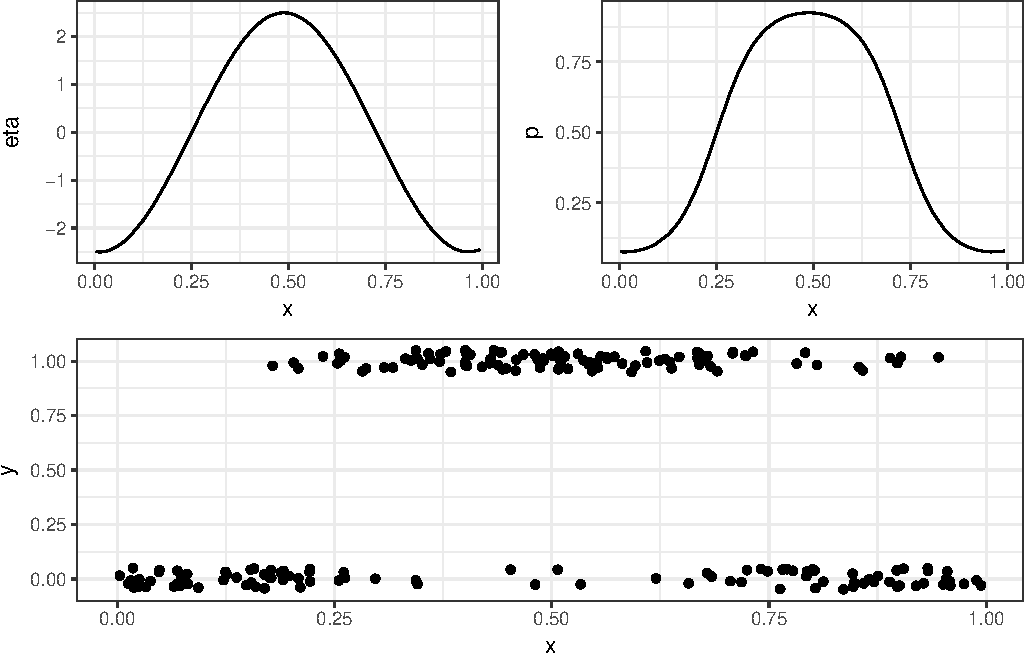
\includegraphics[width=\textwidth]{Lec15_files/figure-beamer/unnamed-chunk-1-1} \end{center}

\end{frame}

\begin{frame}[fragile]{Jags Model\(^*\)}
\protect\hypertarget{jags-model}{}

\scriptoutput

\begin{Shaded}
\begin{Highlighting}[]
\NormalTok{logistic_model =}\StringTok{ "model\{}
\StringTok{  for(i in 1:N) \{}
\StringTok{    y[i] ~ dbern(p[i])}
\StringTok{    logit(p[i]) = beta0 + eta[i]}
\StringTok{    }
\StringTok{    y_hat[i] ~ dbern(p[i])}
\StringTok{    loglik_i[i] = y[i] * log(p[i]) + (1-y[i]) * log(1-p[i])}
\StringTok{  \}}
\StringTok{  loglik = sum(loglik_i)}

\StringTok{  eta ~ dmnorm(rep(0,N), inverse(Sigma))}

\StringTok{  for (i in 1:(length(y)-1)) \{}
\StringTok{    for (j in (i+1):length(y)) \{}
\StringTok{      Sigma[i,j] = sigma2 * exp(- l * d[i,j]))}
\StringTok{      Sigma[j,i] = Sigma[i,j]}
\StringTok{    \}}
\StringTok{  \}}

\StringTok{  for (i in 1:length(y)) \{}
\StringTok{    Sigma[i,i] = sigma2}
\StringTok{  \}  }
\StringTok{  }
\StringTok{  beta0 ~ dnorm(0, 1)}
\StringTok{  sigma2 = 1/tau}
\StringTok{  tau ~ dgamma(1, 2)}
\StringTok{  l ~ dunif(3/0.5, 3/0.01)}
\StringTok{\}"}
\end{Highlighting}
\end{Shaded}

\end{frame}

\begin{frame}{Model Results - Diagnostics}
\protect\hypertarget{model-results---diagnostics}{}

\begin{center}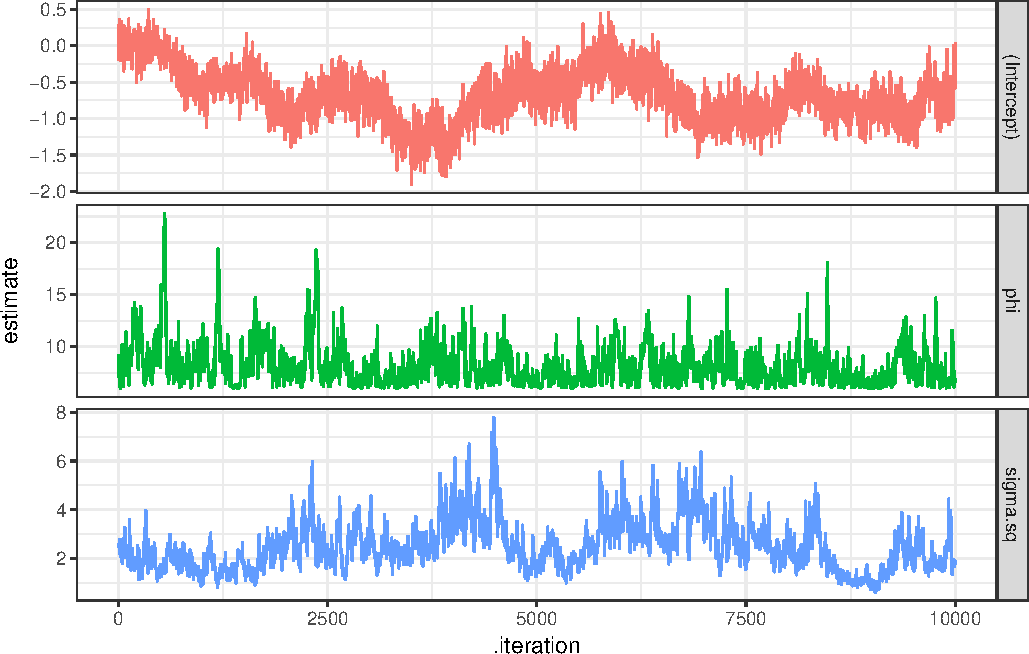
\includegraphics[width=\textwidth]{Lec15_files/figure-beamer/fit_log-1} \end{center}

\end{frame}

\begin{frame}{Model Results - Fit}
\protect\hypertarget{model-results---fit}{}

\begin{center}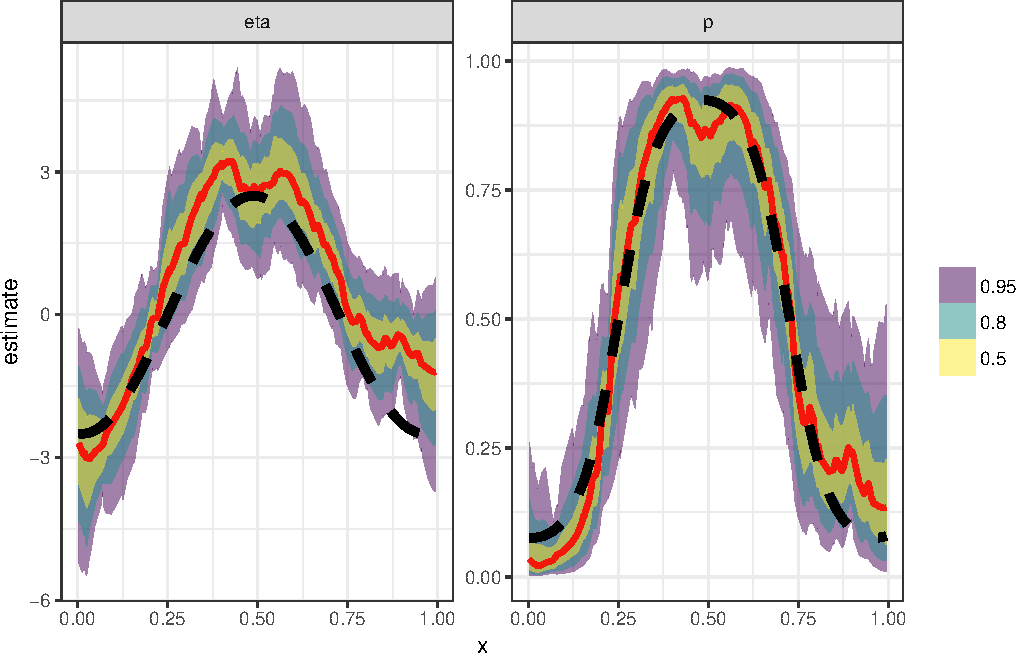
\includegraphics[width=\textwidth]{Lec15_files/figure-beamer/make_pred-1} \end{center}

\end{frame}

\begin{frame}[fragile]{Model vs glm}
\protect\hypertarget{model-vs-glm}{}

\begin{Shaded}
\begin{Highlighting}[]
\NormalTok{g =}\StringTok{ }\KeywordTok{glm}\NormalTok{(y}\OperatorTok{~}\KeywordTok{poly}\NormalTok{(x,}\DecValTok{2}\NormalTok{), }\DataTypeTok{data=}\NormalTok{d, }\DataTypeTok{family=}\StringTok{"binomial"}\NormalTok{)}
\end{Highlighting}
\end{Shaded}

\begin{center}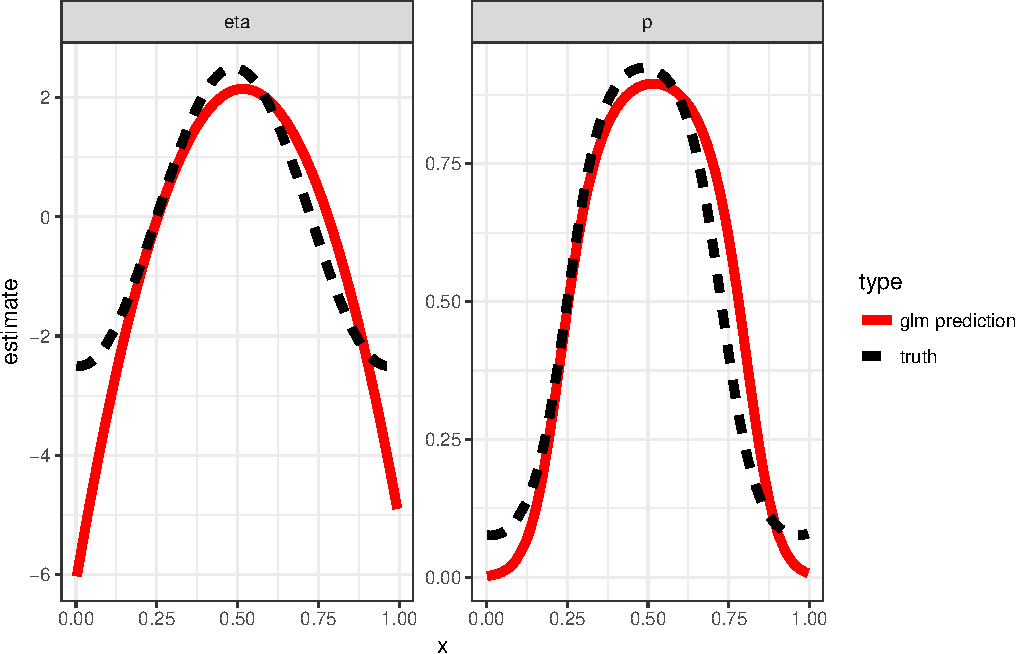
\includegraphics[width=\textwidth]{Lec15_files/figure-beamer/unnamed-chunk-4-1} \end{center}

\end{frame}

\begin{frame}[fragile]{Count data - Polio cases}
\protect\hypertarget{count-data---polio-cases}{}

\texttt{Polio} from the glarma package.

\(~\)

\begin{quote}
This data set gives the monthly number of cases of poliomyelitis in the
U.S. for the years 1970–1983 as reported by the Center for Disease
Control.
\end{quote}

\begin{center}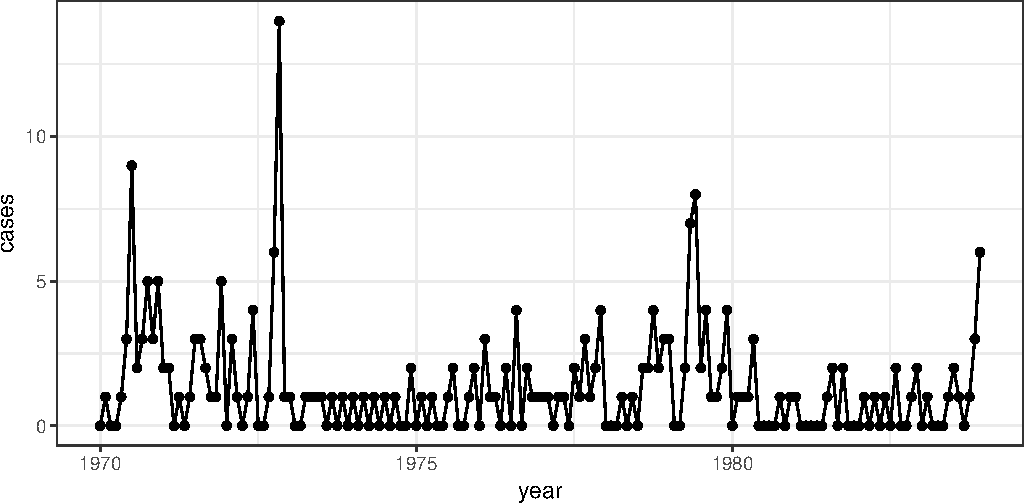
\includegraphics[width=\textwidth]{Lec15_files/figure-beamer/unnamed-chunk-5-1} \end{center}

\end{frame}

\begin{frame}{Polio Model}
\protect\hypertarget{polio-model}{}

\textbf{Model}: \[\begin{aligned}
y_i &\sim \text{Pois}(\lambda_i) \\
\text{log}(\lambda_i) 
  &= \beta_0 + w(\symbf{t}) \\
\end{aligned}\] where \[ w(\symbf{t}) \sim \mathcal{N}(0,\Sigma) \]
\[\{\symbf{\Sigma}\}_{ij} = \sigma^2 \exp(-|\phi \, d_{ij}|)\]

\textbf{Priors}:

\[
\begin{aligned}
\beta_0 &\sim \mathcal{N}(0,1) \\
\phi &\sim \text{Unif}\left(\frac{3}{6}, \frac{3}{1/12}\right)\\
1/\sigma^2 &\sim \text{Gamma}(2,1)
\end{aligned}
\]

\end{frame}

\begin{frame}{Model Results - Diagnostics}
\protect\hypertarget{model-results---diagnostics-1}{}

\begin{center}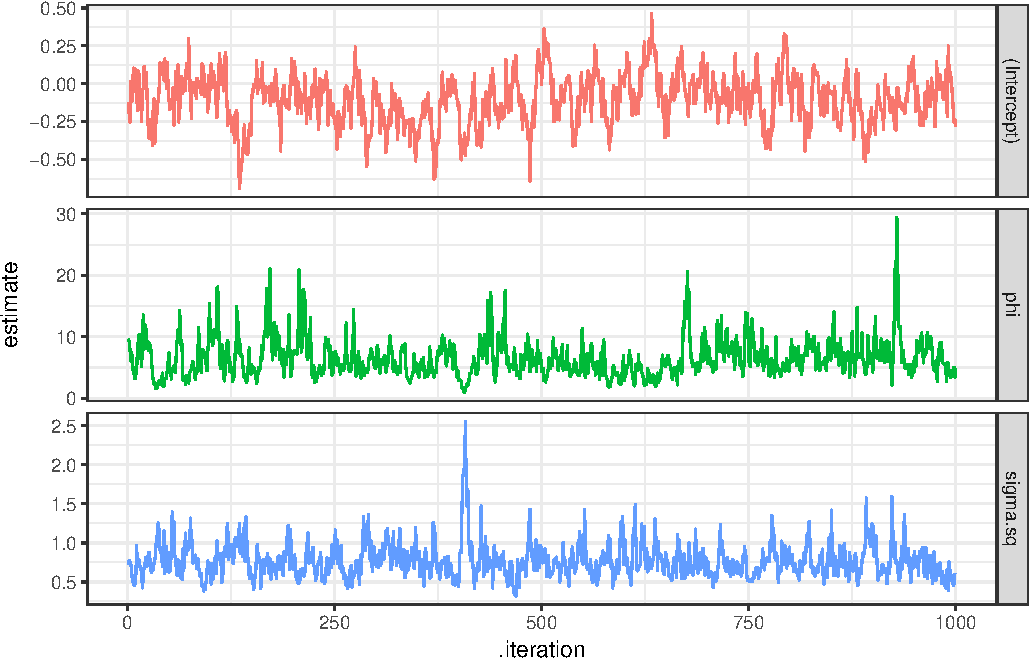
\includegraphics[width=\textwidth]{Lec15_files/figure-beamer/unnamed-chunk-6-1} \end{center}

\end{frame}

\begin{frame}{Model Results - Fit}
\protect\hypertarget{model-results---fit-1}{}

\begin{center}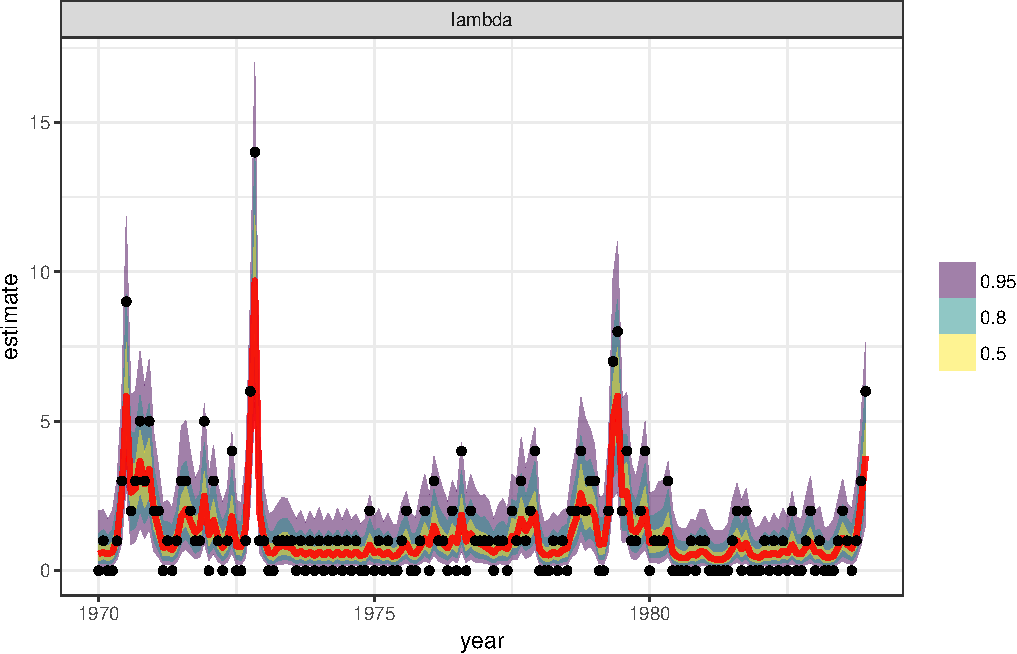
\includegraphics[width=\textwidth]{Lec15_files/figure-beamer/unnamed-chunk-7-1} \end{center}

\end{frame}

\hypertarget{spatial-data-in-r}{%
\section{Spatial data in R}\label{spatial-data-in-r}}

\begin{frame}[fragile,t]{Analysis of geospatial data in R}
\protect\hypertarget{analysis-of-geospatial-data-in-r}{}

R has a rich package ecosystem for read/writing, manipulating, and
analyzing geospatial data.

\vspace{2mm}

Some core packages (CRAN -
\href{http://cran.r-project.org/web/views/Spatial.html}{Spatial task
view}):

\begin{itemize}
\item
  \texttt{sp} - core classes for handling spatial data, additional
  utility functions.
\item
  \texttt{rgdal} - R interface to \texttt{gdal} (Geospatial Data
  Abstraction Library) for reading and writing spatial data.
\item
  \texttt{rgeos} - R interface to \texttt{geos} (Geometry Engine Open
  Source) library for querying and manipulating spatial data. Reading
  and writing WKT.
\item
  \texttt{sf} - Combines the functionality of \texttt{sp},
  \texttt{rgdal}, and \texttt{rgeos} into a single package based on tidy
  priciples.
\item
  \texttt{lwgeom} - additional functionality for \texttt{sf} using
  PostGIS’ liblwgeom.
\item
  \texttt{raster} - classes and tools for handling raster data.
\end{itemize}

\end{frame}

\begin{frame}[fragile,t]{Installing \texttt{sf}}
\protect\hypertarget{installing-sf}{}

This is the hardest part of using the \texttt{sf} package, difficulty
comes from is dependence on several external libraries (\texttt{geos},
\texttt{gdal}, and \texttt{proj}).

\begin{itemize}
\item
  \emph{Windows} - installing from source works when Rtools is installed
  (system requirements are downloaded from rwinlib)
\item
  \emph{MacOS} - install dependencies via homebrew: \texttt{gdal2},
  \texttt{geos}, \texttt{proj}.
\item
  \emph{Linux} - Install development pacakages for GDAL (\textgreater{}=
  2.0.0), GEOS (\textgreater{}= 3.3.0) and Proj.4 (\textgreater{}=
  4.8.0) from your package manager of choice.
\end{itemize}

More specific details are included in the
\href{https://github.com/r-spatial/sf}{repo readme on github}.

\end{frame}

\begin{frame}{Simple Features}
\protect\hypertarget{simple-features}{}

\begin{center}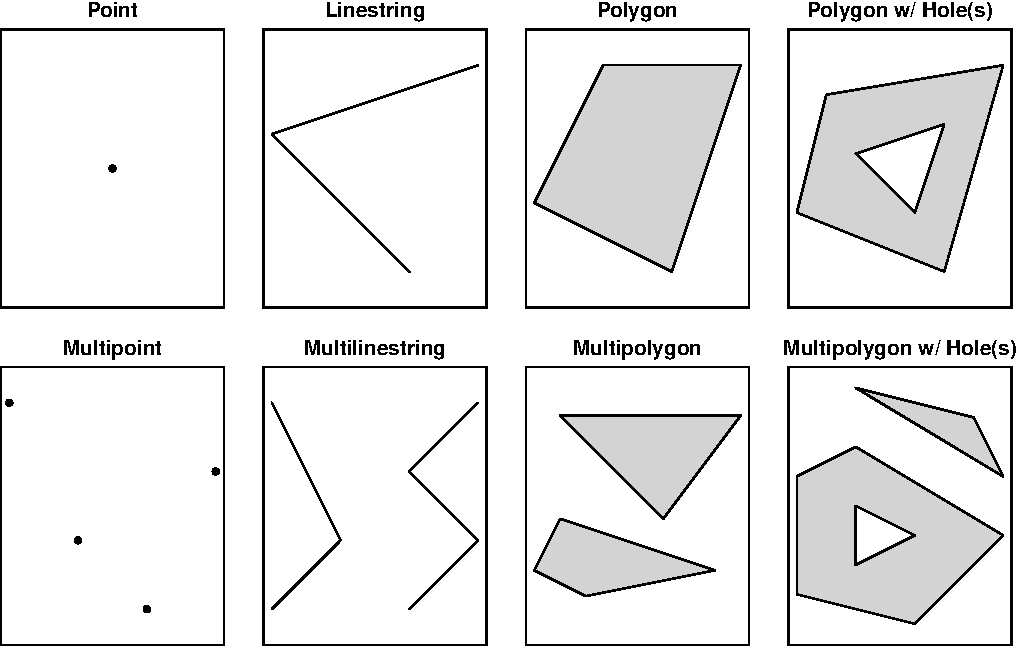
\includegraphics[width=\textwidth]{Lec15_files/figure-beamer/unnamed-chunk-9-1} \end{center}

\end{frame}

\begin{frame}[fragile,t]{Reading, writing, and converting simple
features}
\protect\hypertarget{reading-writing-and-converting-simple-features}{}

\begin{itemize}
\tightlist
\item
  \sout{\texttt{maptools}}

  \begin{itemize}
  \tightlist
  \item
    \sout{\texttt{readShapePoints} / \texttt{writeShapePoints} -
    Shapefile w/ points}
  \item
    \sout{\texttt{readShapeLines} / \texttt{writeShapeLines} - Shapefile
    w/ lines}
  \item
    \sout{\texttt{readShapePoly} / \texttt{writeShapePoly} - Shapefile
    w/ polygons}
  \item
    \sout{\texttt{readShapeSpatial} / \texttt{writeShapeSpatial} -
    Shapefile}
  \end{itemize}
\item
  \sout{\texttt{rgdal}}

  \begin{itemize}
  \tightlist
  \item
    \sout{\texttt{readOGR} / \texttt{writeOGR} - Shapefile, GeoJSON,
    KML, \ldots{}}
  \end{itemize}
\item
  \texttt{rgeos}

  \begin{itemize}
  \tightlist
  \item
    \sout{\texttt{readWKT} / \texttt{writeWKT} - Well Known Text}
  \end{itemize}
\item
  \texttt{sf}

  \begin{itemize}
  \tightlist
  \item
    \texttt{st\_read} / \texttt{st\_write} - Shapefile, GeoJSON, KML,
    \ldots{}
  \item
    \texttt{st\_as\_sfc} / \texttt{st\_as\_wkt} - WKT
  \item
    \texttt{st\_as\_sfc} / \texttt{st\_as\_binary} - WKB
  \item
    \texttt{st\_as\_sfc} / \texttt{as(x,\ "Spatial")} - sp
  \end{itemize}
\end{itemize}

See
\href{https://cran.r-project.org/web/packages/sf/vignettes/sf2.html}{sf
vignette \#2}.

\end{frame}

\hypertarget{geospatial-data-in-the-real-world}{%
\section{Geospatial data in the real
world}\label{geospatial-data-in-the-real-world}}

\begin{frame}{Projections}
\protect\hypertarget{projections}{}

\begin{center}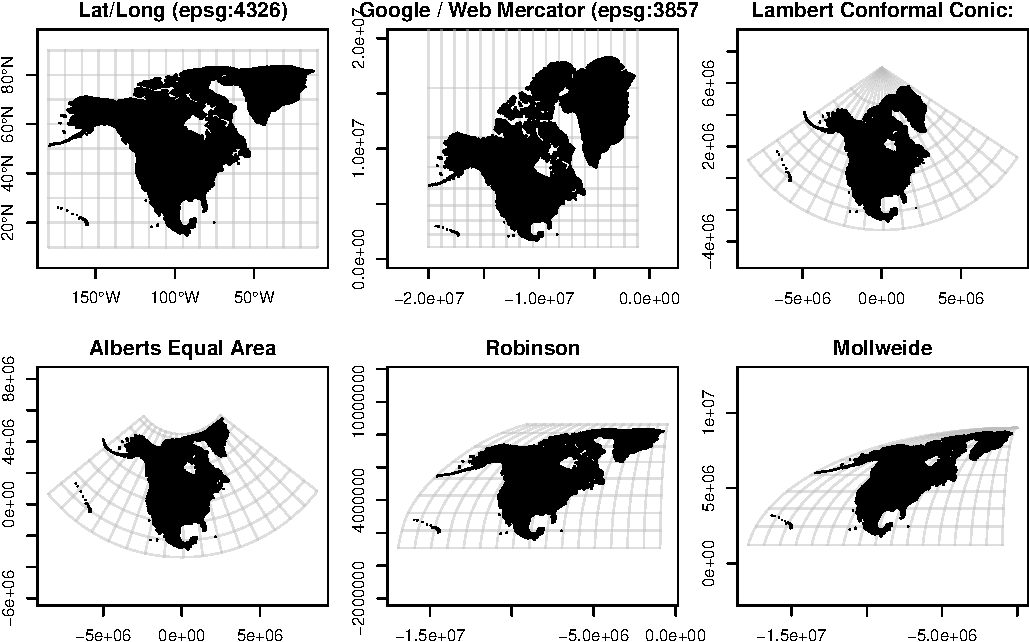
\includegraphics[width=\textwidth]{Lec15_files/figure-beamer/projs-1} \end{center}

\end{frame}

\begin{frame}{Distance on a Sphere}
\protect\hypertarget{distance-on-a-sphere}{}

\begin{center}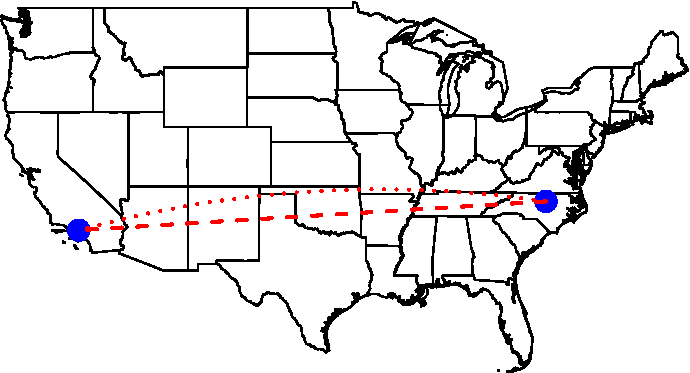
\includegraphics[width=\textwidth]{Lec15_files/figure-beamer/unnamed-chunk-10-1} \end{center}

\end{frame}

\begin{frame}{Dateline}
\protect\hypertarget{dateline}{}

Want to fly from the Western most point in the US to the Eastern most
point?

\begin{center}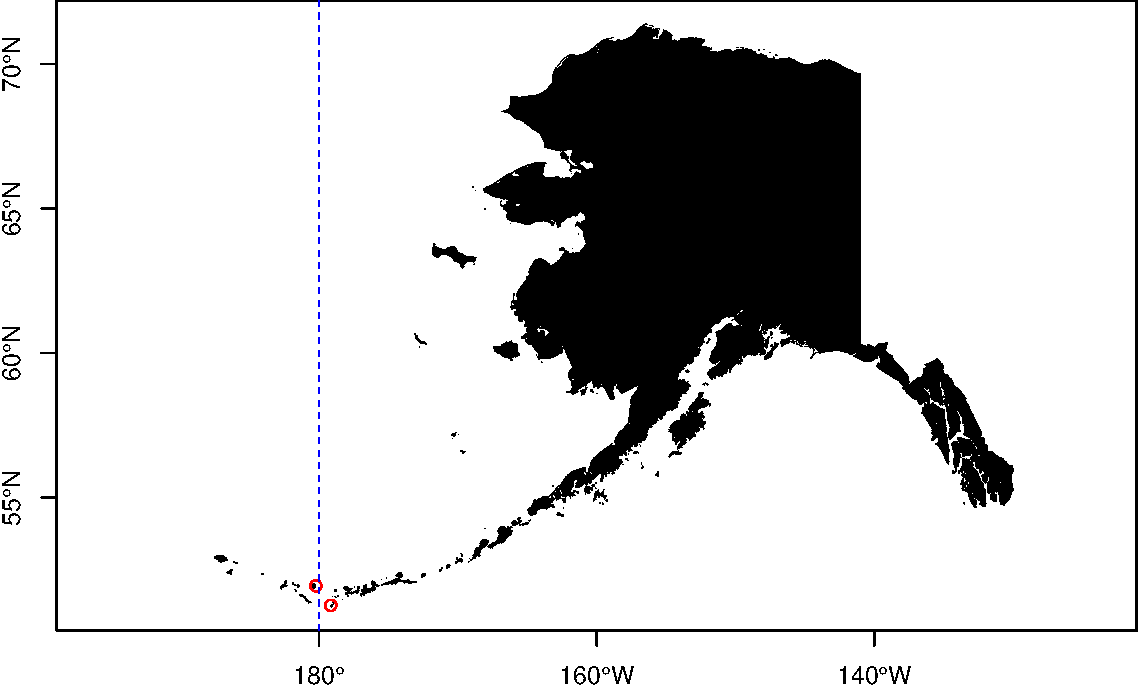
\includegraphics[width=\textwidth]{Lec15_files/figure-beamer/unnamed-chunk-11-1} \end{center}

\end{frame}

\begin{frame}{}
\protect\hypertarget{section}{}

\begin{center}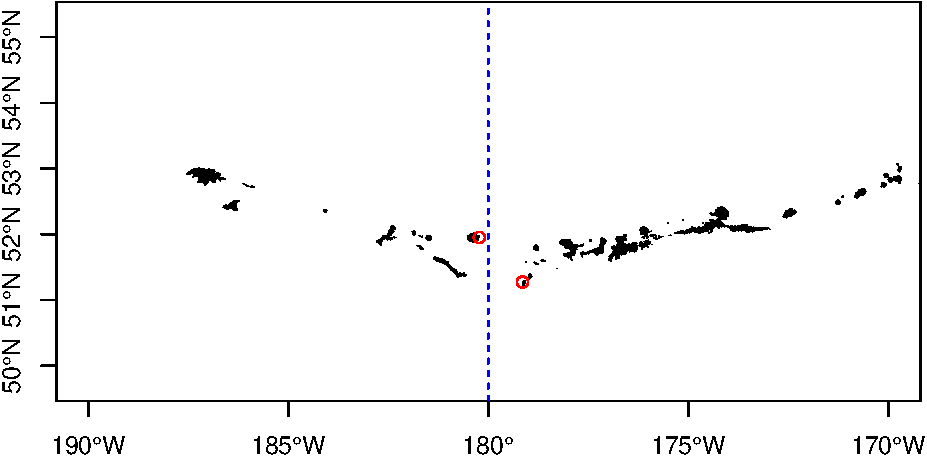
\includegraphics[width=\textwidth]{Lec15_files/figure-beamer/unnamed-chunk-12-1} \end{center}

\end{frame}

\begin{frame}{}
\protect\hypertarget{section-1}{}

\begin{center}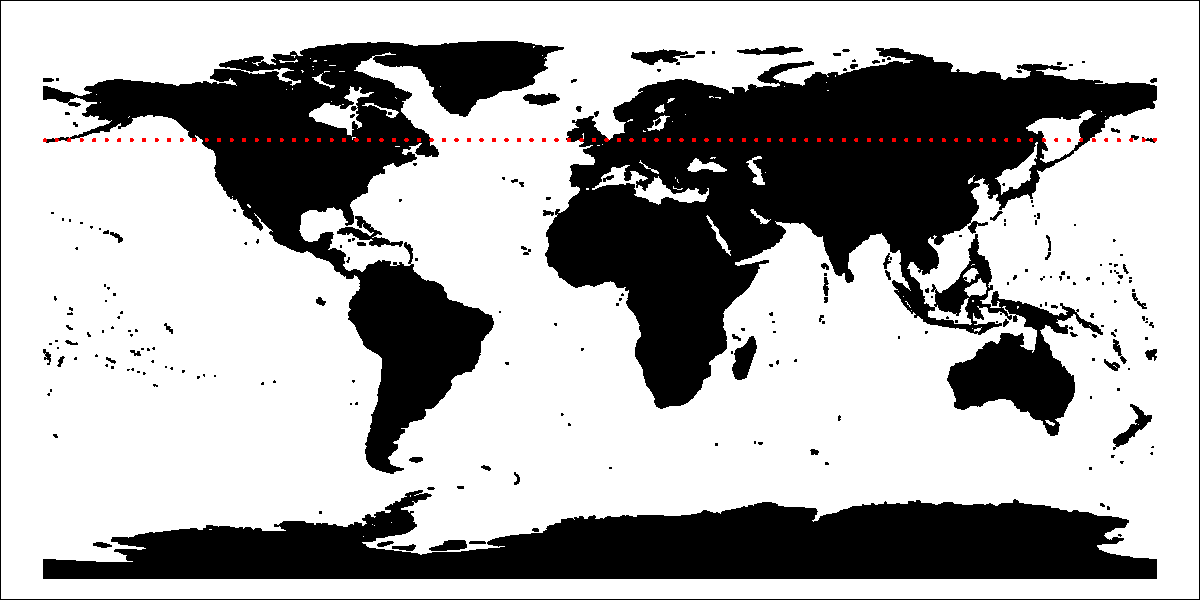
\includegraphics[width=\textwidth]{Lec15_files/figure-beamer/unnamed-chunk-13-1} \end{center}

\end{frame}

\hypertarget{using-sf}{%
\section{\texorpdfstring{Using \texttt{sf}}{Using sf}}\label{using-sf}}

\begin{frame}[fragile,t]{Example data}
\protect\hypertarget{example-data}{}

\scriptoutput

\begin{Shaded}
\begin{Highlighting}[]
\NormalTok{nc  =}\StringTok{ }\KeywordTok{st_read}\NormalTok{(}\StringTok{"../data/gis/nc_counties/"}\NormalTok{, }\DataTypeTok{quiet=}\OtherTok{TRUE}\NormalTok{, }\DataTypeTok{stringsAsFactors=}\OtherTok{FALSE}\NormalTok{)}
\NormalTok{air =}\StringTok{ }\KeywordTok{st_read}\NormalTok{(}\StringTok{"../data/gis/airports/"}\NormalTok{, }\DataTypeTok{quiet=}\OtherTok{TRUE}\NormalTok{, }\DataTypeTok{stringsAsFactors=}\OtherTok{FALSE}\NormalTok{)}
\NormalTok{hwy =}\StringTok{ }\KeywordTok{st_read}\NormalTok{(}\StringTok{"../data/gis/us_interstates/"}\NormalTok{, }\DataTypeTok{quiet=}\OtherTok{TRUE}\NormalTok{, }\DataTypeTok{stringsAsFactors=}\OtherTok{FALSE}\NormalTok{)}

\KeywordTok{tbl_df}\NormalTok{(nc)}
\NormalTok{## # A tibble: 100 x 9}
\NormalTok{##      AREA PERIMETER COUNTYP010 STATE COUNTY    FIPS  STATE_FIPS SQUARE_MIL}
\NormalTok{##     <dbl>     <dbl>      <dbl> <chr> <chr>     <chr> <chr>           <dbl>}
\NormalTok{##  1 0.112       1.61      1994. NC    Ashe Cou~ 37009 37               429.}
\NormalTok{##  2 0.0616      1.35      1996. NC    Alleghan~ 37005 37               236.}
\NormalTok{##  3 0.140       1.77      1998. NC    Surry Co~ 37171 37               539.}
\NormalTok{##  4 0.0891      1.43      1999. NC    Gates Co~ 37073 37               342.}
\NormalTok{##  5 0.0687      4.43      2000. NC    Currituc~ 37053 37               264.}
\NormalTok{##  6 0.119       1.40      2001. NC    Stokes C~ 37169 37               456.}
\NormalTok{##  7 0.0626      2.11      2002. NC    Camden C~ 37029 37               241.}
\NormalTok{##  8 0.115       1.46      2003. NC    Warren C~ 37185 37               444.}
\NormalTok{##  9 0.143       2.40      2004. NC    Northamp~ 37131 37               551.}
\NormalTok{## 10 0.0925      1.81      2005. NC    Hertford~ 37091 37               356.}
\NormalTok{## # ... with 90 more rows, and 1 more variable: geometry <sf_geometry}
\NormalTok{## #   [degree]>}
\end{Highlighting}
\end{Shaded}

\end{frame}

\begin{frame}[fragile,t]{}
\protect\hypertarget{section-2}{}

\scriptoutput

\begin{Shaded}
\begin{Highlighting}[]
\KeywordTok{tbl_df}\NormalTok{(air)}
\NormalTok{## # A tibble: 940 x 17}
\NormalTok{##    AIRPRTX010 FEATURE ICAO  IATA  AIRPT_NAME CITY  STATE STATE_FIPS COUNTY}
\NormalTok{##         <dbl> <chr>   <chr> <chr> <chr>      <chr> <chr> <chr>      <chr> }
\NormalTok{##  1         0. AIRPORT KGON  GON   GROTON-NE~ GROT~ CT    09         NEW L~}
\NormalTok{##  2         3. AIRPORT K6S5  6S5   RAVALLI C~ HAMI~ MT    30         RAVAL~}
\NormalTok{##  3         4. AIRPORT KMHV  MHV   MOJAVE AI~ MOJA~ CA    06         KERN  }
\NormalTok{##  4         6. AIRPORT KSEE  SEE   GILLESPIE~ SAN ~ CA    06         SAN D~}
\NormalTok{##  5         7. AIRPORT KFPR  FPR   ST LUCIE ~ FORT~ FL    12         ST LU~}
\NormalTok{##  6         8. AIRPORT KRYY  RYY   COBB COUN~ ATLA~ GA    13         COBB  }
\NormalTok{##  7        10. AIRPORT KMKL  MKL   MC KELLAR~ JACK~ TN    47         MADIS~}
\NormalTok{##  8        11. AIRPORT KCCR  CCR   BUCHANAN ~ CONC~ CA    06         CONTR~}
\NormalTok{##  9        13. AIRPORT KJYO  JYO   LEESBURG ~ LEES~ VA    51         LOUDO~}
\NormalTok{## 10        15. AIRPORT KCAD  CAD   WEXFORD C~ CADI~ MI    26         WEXFO~}
\NormalTok{## # ... with 930 more rows, and 8 more variables: FIPS <chr>, TOT_ENP <dbl>,}
\NormalTok{## #   LATITUDE <dbl>, LONGITUDE <dbl>, ELEV <dbl>, ACT_DATE <chr>,}
\NormalTok{## #   CNTL_TWR <chr>, geometry <sf_geometry [degree]>}
\end{Highlighting}
\end{Shaded}

\end{frame}

\begin{frame}[fragile,t]{}
\protect\hypertarget{section-3}{}

\scriptoutput

\begin{Shaded}
\begin{Highlighting}[]
\KeywordTok{tbl_df}\NormalTok{(hwy)}
\NormalTok{## # A tibble: 233 x 4}
\NormalTok{##    ROUTE_NUM DIST_MILES DIST_KM                       geometry}
\NormalTok{##    <chr>          <dbl>   <dbl>              <sf_geometry [m]>}
\NormalTok{##  1 I10          2449.   3941.   MULTILINESTRING ((-1881200 ...}
\NormalTok{##  2 I105           20.8    33.4  MULTILINESTRING ((-1910156 ...}
\NormalTok{##  3 I110           41.4    66.6  MULTILINESTRING ((1054139 3...}
\NormalTok{##  4 I115            1.58    2.55 MULTILINESTRING ((-1013796 ...}
\NormalTok{##  5 I12            85.3   137.   MULTILINESTRING ((680741.7 ...}
\NormalTok{##  6 I124            1.73    2.79 MULTILINESTRING ((1201467 3...}
\NormalTok{##  7 I126            3.56    5.72 MULTILINESTRING ((1601502 3...}
\NormalTok{##  8 I129            3.10    4.99 MULTILINESTRING ((217446 47...}
\NormalTok{##  9 I135           96.3   155.   MULTILINESTRING ((96922.97 ...}
\NormalTok{## 10 I15          1436.   2311.   MULTILINESTRING ((-882875.7...}
\NormalTok{## # ... with 223 more rows}
\end{Highlighting}
\end{Shaded}

\end{frame}

\begin{frame}[fragile]{\texttt{sf} classes}
\protect\hypertarget{sf-classes}{}

\scriptoutput

\begin{Shaded}
\begin{Highlighting}[]
\KeywordTok{str}\NormalTok{(nc)}
\NormalTok{## Classes 'sf' and 'data.frame':   100 obs. of  9 variables:}
\NormalTok{##  $ AREA      : num  0.1118 0.0616 0.1402 0.0891 0.0687 ...}
\NormalTok{##  $ PERIMETER : num  1.61 1.35 1.77 1.43 4.43 ...}
\NormalTok{##  $ COUNTYP010: num  1994 1996 1998 1999 2000 ...}
\NormalTok{##  $ STATE     : chr  "NC" "NC" "NC" "NC" ...}
\NormalTok{##  $ COUNTY    : chr  "Ashe County" "Alleghany County" "Surry County" "Gates County" ...}
\NormalTok{##  $ FIPS      : chr  "37009" "37005" "37171" "37073" ...}
\NormalTok{##  $ STATE_FIPS: chr  "37" "37" "37" "37" ...}
\NormalTok{##  $ SQUARE_MIL: num  429 236 539 342 264 ...}
\NormalTok{##  $ geometry  :sfc_MULTIPOLYGON of length 100; first list element: List of 1}
\NormalTok{##   ..$ :List of 1}
\NormalTok{##   .. ..$ : num [1:1030, 1:2] -81.7 -81.7 -81.7 -81.6 -81.6 ...}
\NormalTok{##   ..- attr(*, "class")= chr  "XY" "MULTIPOLYGON" "sfg"}
\NormalTok{##  - attr(*, "sf_column")= chr "geometry"}
\NormalTok{##  - attr(*, "agr")= Factor w/ 3 levels "constant","aggregate",..: NA NA NA NA NA NA NA NA}
\NormalTok{##   ..- attr(*, "names")= chr  "AREA" "PERIMETER" "COUNTYP010" "STATE" ...}

\KeywordTok{class}\NormalTok{(nc)}
\NormalTok{## [1] "sf"         "data.frame"}

\KeywordTok{class}\NormalTok{(nc}\OperatorTok{$}\NormalTok{geometry)}
\NormalTok{## [1] "sfc_MULTIPOLYGON" "sfc"}

\KeywordTok{class}\NormalTok{(nc}\OperatorTok{$}\NormalTok{geometry[[}\DecValTok{1}\NormalTok{]])}
\NormalTok{## [1] "XY"           "MULTIPOLYGON" "sfg"}
\end{Highlighting}
\end{Shaded}

\end{frame}

\begin{frame}[fragile,t]{Projections}
\protect\hypertarget{projections-1}{}

\begin{Shaded}
\begin{Highlighting}[]
\KeywordTok{st_crs}\NormalTok{(nc)}\OperatorTok{$}\NormalTok{proj4string}
\NormalTok{## [1] "+proj=longlat +datum=NAD83 +no_defs"}
\KeywordTok{st_crs}\NormalTok{(air)}\OperatorTok{$}\NormalTok{proj4string}
\NormalTok{## [1] "+proj=longlat +datum=NAD83 +no_defs"}
\KeywordTok{st_crs}\NormalTok{(hwy)}\OperatorTok{$}\NormalTok{proj4string}
\NormalTok{## [1] "+proj=utm +zone=15 +datum=NAD83 +units=m +no_defs"}
\end{Highlighting}
\end{Shaded}

\begin{center}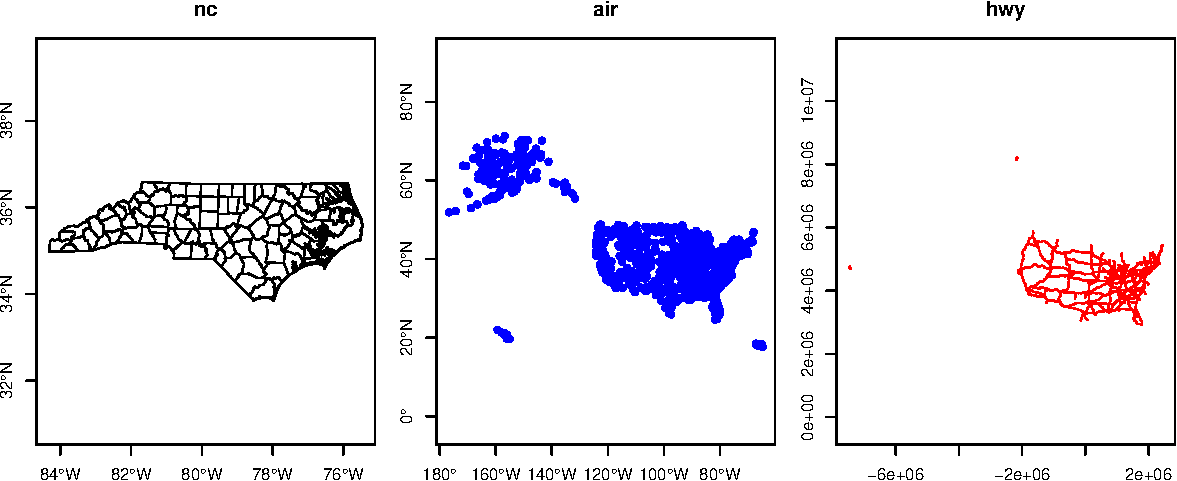
\includegraphics[width=\textwidth]{Lec15_files/figure-beamer/unnamed-chunk-19-1} \end{center}

\end{frame}

\begin{frame}{UTM Zones}
\protect\hypertarget{utm-zones}{}

\begin{center}
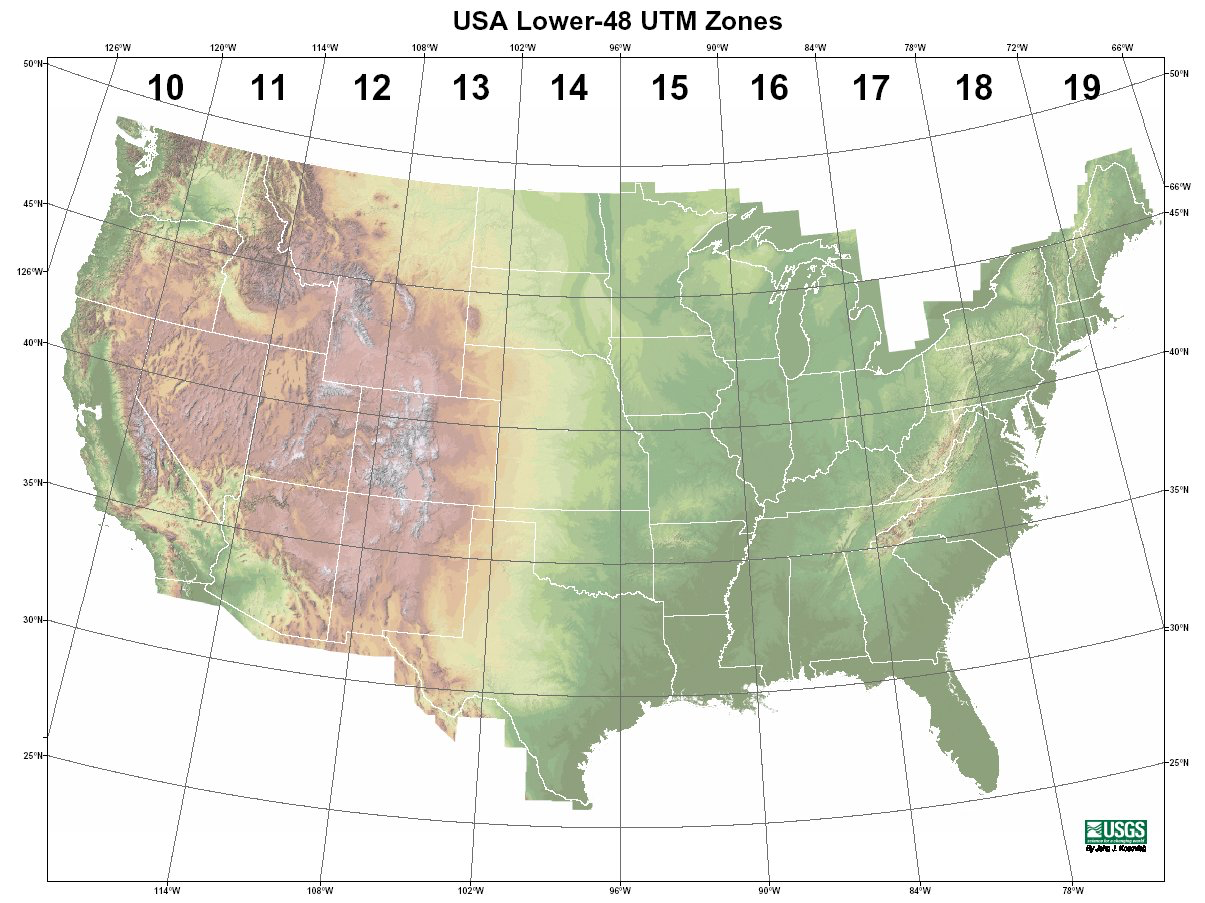
\includegraphics[width=0.9\textwidth]{figs/UTM_Zones.png}
\end{center}

\end{frame}

\begin{frame}[fragile]{Lat/Long}
\protect\hypertarget{latlong}{}

\begin{Shaded}
\begin{Highlighting}[]
\NormalTok{nc_ll =}\StringTok{ }\NormalTok{nc}
\NormalTok{air_ll =}\StringTok{ }\NormalTok{air}
\NormalTok{hwy_ll =}\StringTok{ }\NormalTok{lwgeom}\OperatorTok{::}\KeywordTok{st_transform_proj}\NormalTok{(hwy, }\KeywordTok{st_crs}\NormalTok{(nc)}\OperatorTok{$}\NormalTok{proj4string)}
\end{Highlighting}
\end{Shaded}

\begin{center}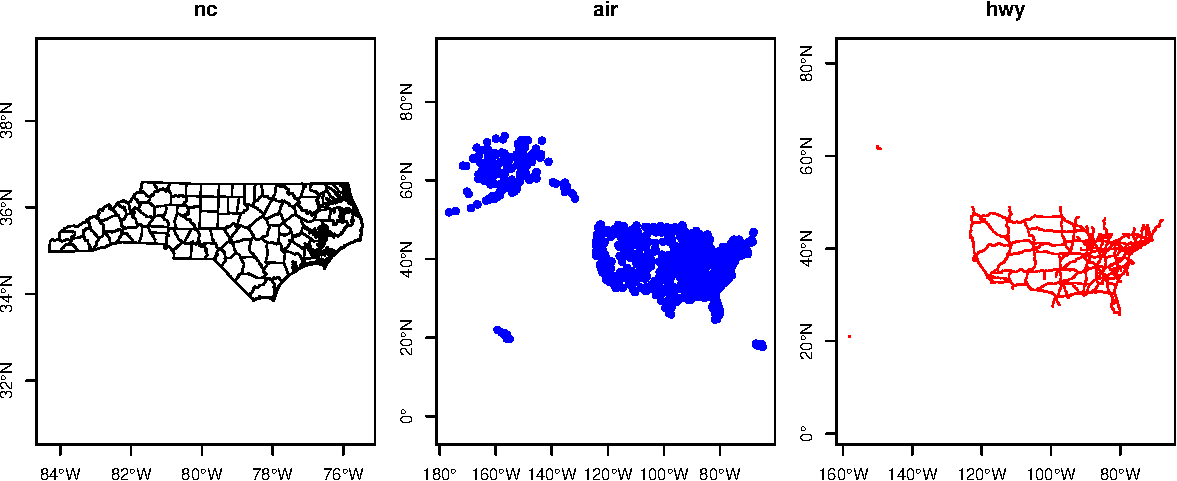
\includegraphics[width=\textwidth]{Lec15_files/figure-beamer/unnamed-chunk-21-1} \end{center}

\end{frame}

\begin{frame}[fragile]{UTM}
\protect\hypertarget{utm}{}

\begin{Shaded}
\begin{Highlighting}[]
\NormalTok{nc_utm =}\StringTok{ }\NormalTok{lwgeom}\OperatorTok{::}\KeywordTok{st_transform_proj}\NormalTok{(nc, }\KeywordTok{st_crs}\NormalTok{(hwy)}\OperatorTok{$}\NormalTok{proj4string)}
\NormalTok{air_utm =}\StringTok{ }\NormalTok{lwgeom}\OperatorTok{::}\KeywordTok{st_transform_proj}\NormalTok{(air, }\KeywordTok{st_crs}\NormalTok{(hwy)}\OperatorTok{$}\NormalTok{proj4string)}
\NormalTok{hwy_utm =}\StringTok{ }\NormalTok{hwy}
\end{Highlighting}
\end{Shaded}

\begin{center}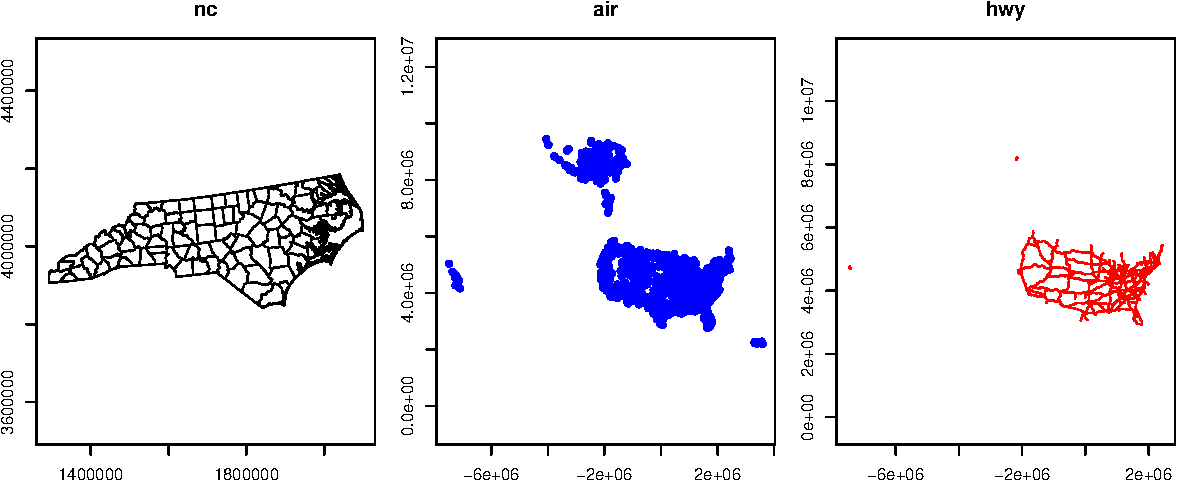
\includegraphics[width=\textwidth]{Lec15_files/figure-beamer/unnamed-chunk-23-1} \end{center}

\end{frame}

\begin{frame}{Comparison}
\protect\hypertarget{comparison}{}

\begin{center}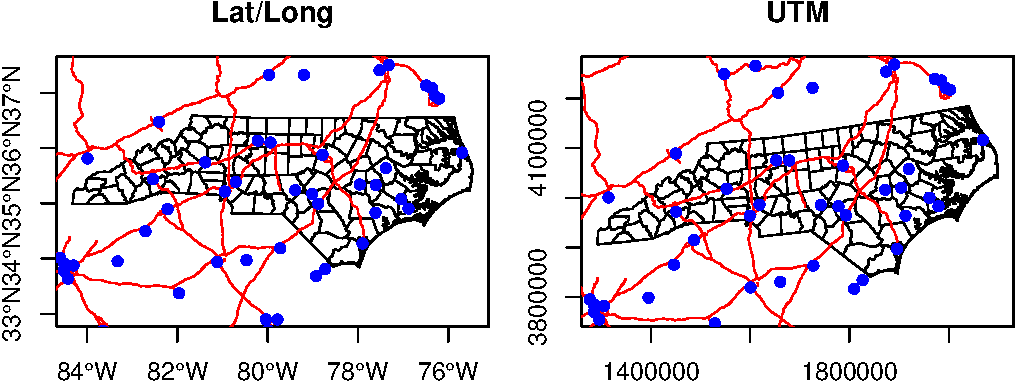
\includegraphics[width=\textwidth]{Lec15_files/figure-beamer/unnamed-chunk-24-1} \end{center}

\end{frame}

\hypertarget{geometry-predicates}{%
\section{Geometry Predicates}\label{geometry-predicates}}

\begin{frame}{DE-9IM}
\protect\hypertarget{de-9im}{}

\begin{center}
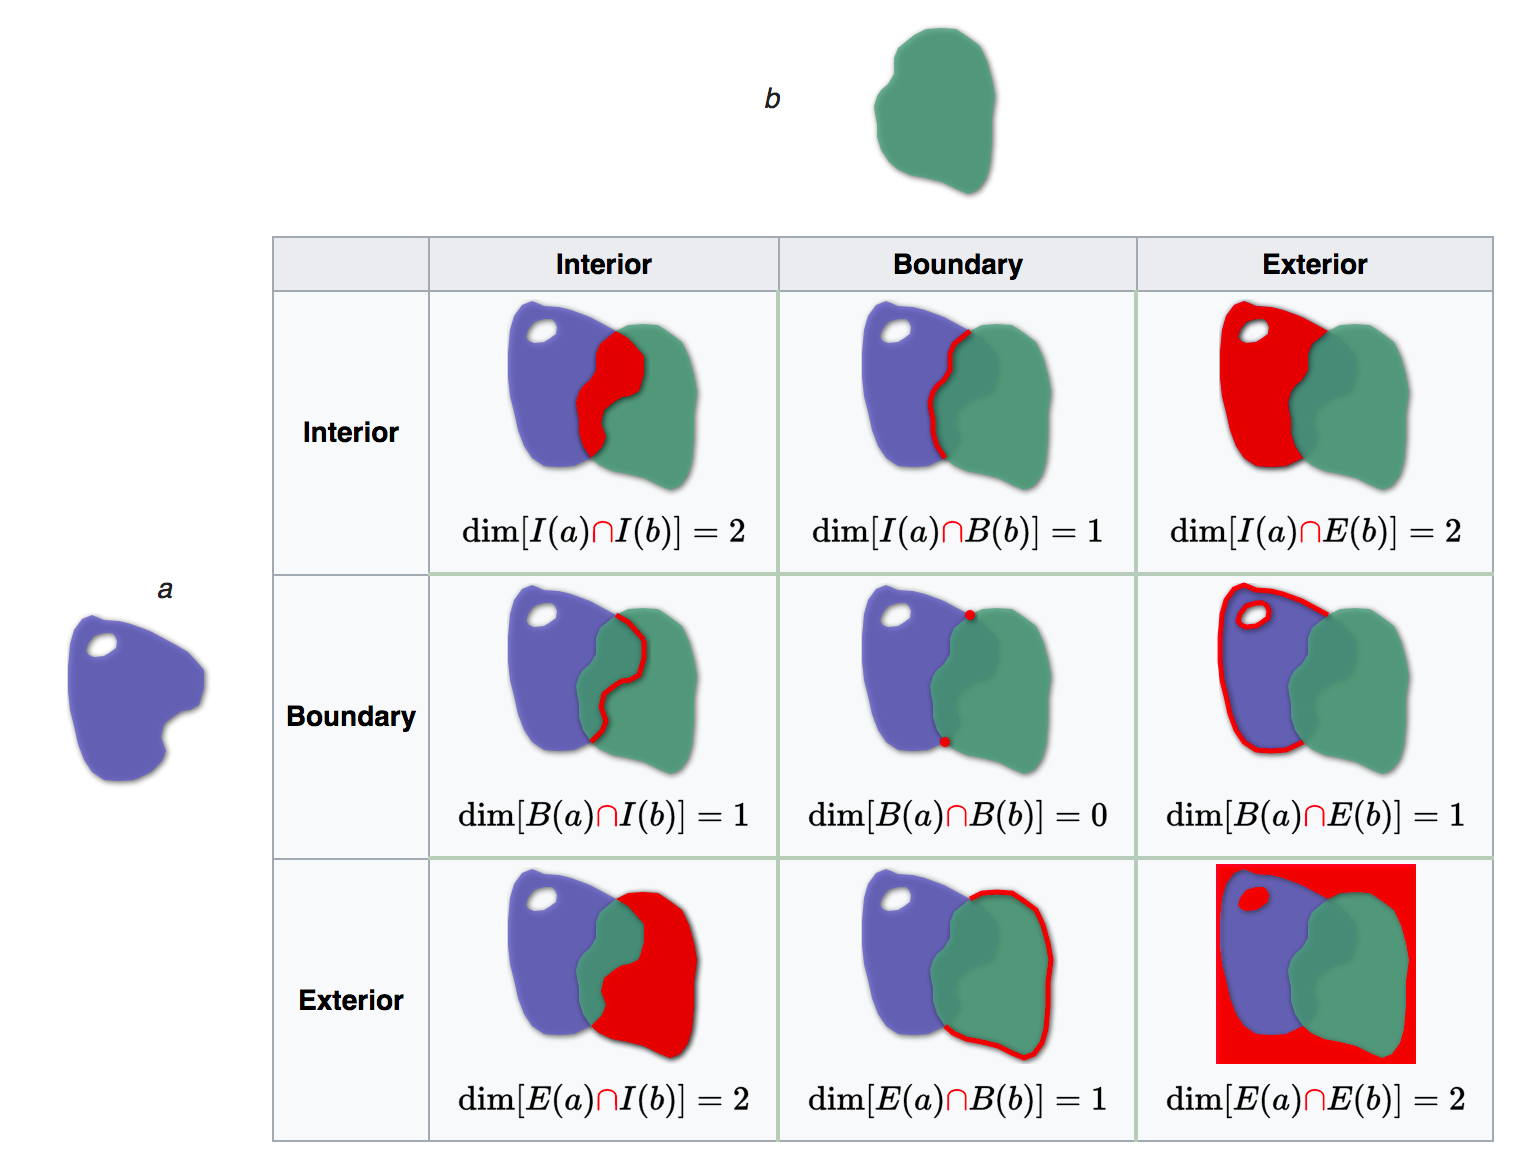
\includegraphics[width=0.95\textwidth]{figs/de_9im.png}
\end{center}

\end{frame}

\begin{frame}{Spatial predicates}
\protect\hypertarget{spatial-predicates}{}

\begin{center}
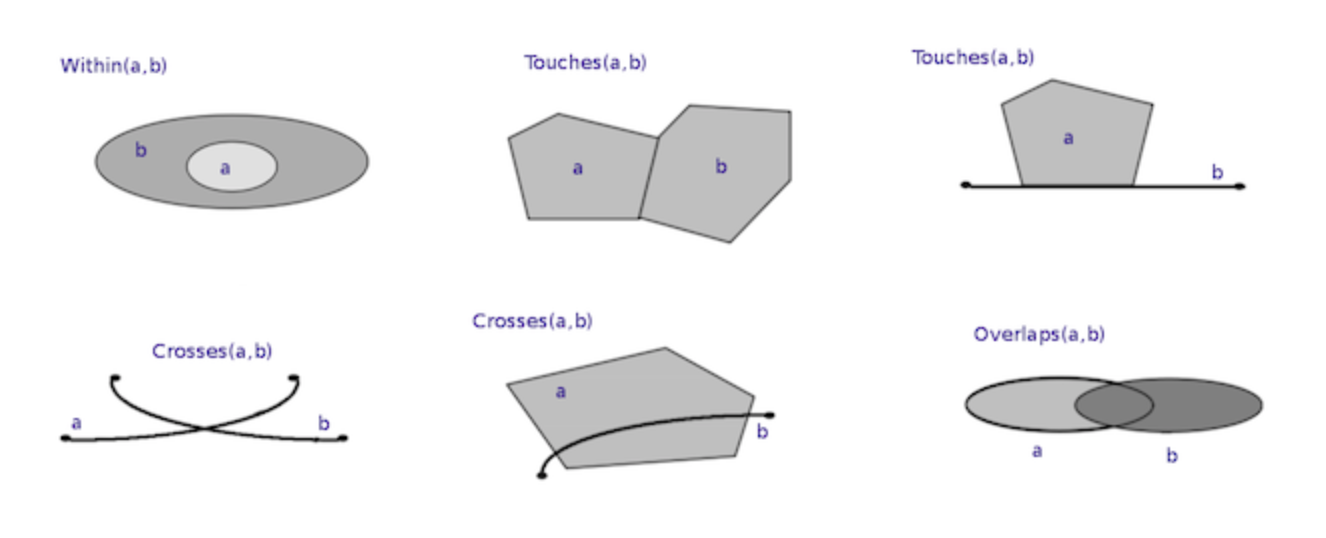
\includegraphics[width=0.75\textwidth]{figs/predicates.png}
\end{center}

\footnotesize

\hspace*{-4pt}\makebox[\linewidth][c]{
\begin{tabular}{lll}

st\_within(a,b) & & st\_touches(a,b) \\

$\begin{bmatrix} T & * & F \\ * & * & F \\ * & * & * \end{bmatrix}$ & &
$\begin{bmatrix} F & T & * \\ * & * & * \\ * & * & * \end{bmatrix} \cup 
\begin{bmatrix} F & * & * \\ T & * & * \\ * & * & * \end{bmatrix} \cup 
\begin{bmatrix} F & * & * \\ * & T & * \\ * & * & * \end{bmatrix}$ \\

\\

st\_crosses(a,b) & & st\_overlaps(a,b) ($\text{dim}(a) = \text{dim}(b)$) \\

$\overset{\text{If dim}(a) < \text{dim}(b)}{\begin{bmatrix} T & * & T \\ * & * & * \\ * & * & * \end{bmatrix}} ~~~
\overset{\text{If dim}(a) > \text{dim}(b)}{\begin{bmatrix} T & * & * \\ * & * & * \\ T & * & * \end{bmatrix}} ~~~
\overset{\text{If dim}(any) = 1}{\begin{bmatrix} 0 & * & * \\ * & * & * \\ * & * & * \end{bmatrix}}$ & &
$\overset{\text{If dim} \in \{0,2\}}{\begin{bmatrix} T & * & T \\ * & * & * \\ T & * & * \end{bmatrix}} ~~~
\overset{\text{If dim} = 1}{\begin{bmatrix} 1 & * & T \\ * & * & * \\ T & * & * \end{bmatrix}}$ \\
\end{tabular}
}

\end{frame}

\begin{frame}[fragile]{Sparse vs Full Results}
\protect\hypertarget{sparse-vs-full-results}{}

\scriptsize

\begin{Shaded}
\begin{Highlighting}[]
\KeywordTok{st_intersects}\NormalTok{(nc[}\DecValTok{20}\OperatorTok{:}\DecValTok{30}\NormalTok{,], air) }\OperatorTok\StringTok{ }\KeywordTok{str}\NormalTok{()}
\NormalTok{## although coordinates are longitude/latitude, st_intersects assumes that they are planar}
\NormalTok{## List of 11}
\NormalTok{##  $ : int(0) }
\NormalTok{##  $ : int(0) }
\NormalTok{##  $ : int(0) }
\NormalTok{##  $ : int(0) }
\NormalTok{##  $ : int(0) }
\NormalTok{##  $ : int 268}
\NormalTok{##  $ : int 717}
\NormalTok{##  $ : int(0) }
\NormalTok{##  $ : int(0) }
\NormalTok{##  $ : int(0) }
\NormalTok{##  $ : int(0) }
\NormalTok{##  - attr(*, "predicate")= chr "intersects"}
\NormalTok{##  - attr(*, "region.id")= chr [1:11] "20" "21" "22" "23" ...}
\NormalTok{##  - attr(*, "ncol")= int 940}
\NormalTok{##  - attr(*, "class")= chr "sgbp"}
\end{Highlighting}
\end{Shaded}

\begin{Shaded}
\begin{Highlighting}[]
\KeywordTok{st_intersects}\NormalTok{(nc, air, }\DataTypeTok{sparse=}\OtherTok{FALSE}\NormalTok{) }\OperatorTok\StringTok{ }\KeywordTok{str}\NormalTok{()}
\NormalTok{## although coordinates are longitude/latitude, st_intersects assumes that they are planar}
\NormalTok{##  logi [1:100, 1:940] FALSE FALSE FALSE FALSE FALSE FALSE ...}
\end{Highlighting}
\end{Shaded}

\end{frame}

\begin{frame}[t]{Examples}
\protect\hypertarget{examples}{}

\begin{itemize}
\item
  Which counties are adjacent to Durham County?
\item
  Which counties have more than 4 neighbors?
\item
  Which counties have an airport?
\end{itemize}

\end{frame}

\end{document}
